\documentclass{article}

\usepackage{graphicx}
\usepackage{hyperref}
\hypersetup{
    colorlinks=true,
    linkcolor=black,
    filecolor=black,
    citecolor=black,    
    urlcolor=black,
}
\graphicspath{ {../figures} }

\title{An Exploration of Analysis Methods on Predictive Models of Student Success}
\author{Alex Beckwith\\\\University of New Hampshire}
\date{May 2023}
\begin{document}

\maketitle
\newpage

\tableofcontents

\begin{abstract}
    Machine learning models are not always evaluated with statistical rigor. 
    This can lead to inferential flaws when assumptions are made about the underlying and performance data, especially when cross-validation is used. 
    In this paper, a Bayesian method of model evaluation is compared to a non-parametric frequentist method. 
    In addition, a metric for analyzing the fairness of a particular algorithm is tested. 

    The evaluation techniques were applied to a dataset of student and course data made available by the Open University. 
    A system was built to train and test predictive models of student success. 
    The aim was to predict students at risk of failing or withdrawing from a course using the first 30 days of data extracted from the virtual learning environment. 
    In an applied setting, these predictions could be used to direct additional resources to at-risk students. 

    The project included creating a database to cleanse, transform, and analyze the dataset. 
    Features were engineered to use as predictive inputs using a combination of exploratory analysis and inspiration from research. 
    Four different subsets of input features were applied to nine different classification algorithms. 
    Both randomized and exhaustive hyperparameter tuning procedures were experimented with, which created hundreds of distinct hyperparameter settings.  

    The Bayesian strategy provided more conclusive results by determining a “region of practical equivalence” as opposed to an inability to reject the null hypothesis. 
    The results were similar to findings from research, which typically found tree-based ensemble methods in the upper-equivalence region. 

    The proposed metric for predictive fairness is called the Absolute Between Receiver Operating Characteristic Area (ABROCA). 
    This metric was first introduced at the 2019 International Learning Analytics and Knowledge Conference. 
    A significant relationship between ABROCA and the gender ratio of a course as well as between ABROCA and the ratio of students in a course identifying as having a disability. 
    No significant relationship was found between ABROCA and overall model performance. 
\end{abstract}
\newpage

\section{Introduction}
        When creating a predictive model to solve a problem, many different formulations and algorithms are typically tested.
        Datasets can be vast and complex, so the "see what sticks" strategy is often a good first step.

        Selecting the appropriate model to deploy should involve the consideration of many factors.
        Predictive performance is important, but simply picking the model with the highest mean accuracy is not a valid strategy.
        Statistical evaluation enables confident decisionmaking, which frees the researcher to address other considerations.

        In this project, I applied the best practices from my research on model evaluation to a publicly-available dataset provided by an educational institution.
        I created a system that generates models that attempt to predict students who are likely to fail or drop out of a course.
        The practical application of the final model's predictions would be to target vulnerable students with interventions to increase their likelihood of course completion. 

        Using the results of the model testing, I show why a Bayesian approach is better for the evaluation of predictive models. 
        In addition, I implement a new metric for testing model fairness. 
        I affirm the results of the researchers who proposed the metric, showing that it is strongly correlated with a decrease in predictive fairness while showing scant correlation with predictive performance.
    
    \subsection{Research Questions}
        \begin{enumerate}
            \item Which models and featuresets are best at predicting student outcomes?
            \item How do the results differ when evaluated using naive, frequentist, and Bayesian procedures?
            \item Is there an association between model predictive performance and Absolute Between Receiver Operating Characteristic Area (ABROCA)?
        \end{enumerate}
    

\section{Previous Research}
    \subsection{Learning Analytics}
        This project falls squarely within the interdiciplinary field of Educational Data Science (EDS), which itself is the union of Learning Analytics (LA) and Educational Data Mining (EDM).
        EDM is primarily concerned with the development of methods for exploring the unique types of data that come from education environments \cite{educate2019}.
        LA is focused on the analysis of learners and the optimization of the learning process \cite{educate2019}.
        The first EDM and LA-specific conferences took place in 2008 and 2011, respectively. 
        All three have roots in statistics, education, and computer science, and all three use data to address important educational questions and issues.
        For a more comprehensive review of these fields, please refer to \cite{educate2007,educate2010,educate2019}.

    \subsection{Modeling Student Performance}
        \subsubsection{Predictions}
            One of the most common topics in LA and EDM is the creation of machine learning models to predict student behavior and performance.
            Researchers most often frame problems in the context of classification and regression problems \cite{educate2007,educate2010,educate2019}.
            Within the subset of research on classification and regression models, the most common features to predict were outcomes and scores \cite{compare2015}.
            In the context of a course, that might be whether the student passes or their final grade.
            One could also consider the context of a single problem, such as the student's most likely answer or the probability of being correct/incorrect \cite{explore2021}.
            The most effective algorithms for classification problems of these type in my research were tree-based ensemble methods.

        \subsubsection{Model Types}
            In my research, the models which best predicted student performance tended to be tree-based ensemble methods \cite{explore2021,engage2014,assign2021esteban}.
            Tree-based methods were also the most commonly seen type of model, followed by linear and logistic regression \cite{assign2021esteban}.
            Other common models include support vector machines, k-nearest neighbors, and naive Bayes.
            Research related to the utilization of deep learning is not uncommon \cite{explore2021,assign2021esteban}, though I wasn't able to find a resource which utilized a neural network that significantly outperformed simpler methods.

    \subsection{Student Data}
        \subsubsection{Sources}
            The most common sources of student data came from Massively Open Online Courses (MOOCs), Intelligent Tutoring Systems (ITS) and other computer-based platforms,
            though a great deal of research has also been conducted using data from traditional classrooms \cite{educate2019,early2021,assign2021esteban,explore2015}.
            Especially since the pandemic of the early 2020s, many students have experienced educational systems which blend the two.
            Blended sources of learning data would benefit from additional research \cite{educate2019,early2021}.

        \subsubsection{Featuresets}
            The most common featuresets for predicting student outcomes are academic, demographic, and behavioral \cite{engage2014,eval2018,early2019,assign2021esteban,compare2015}.
            Academic includes information about assessments and assignments \cite{assign2021esteban}.
            Behavioral data is often the logs from student interactions with the Virtual Learning Environment (VLE) \cite{early2019,assign2021esteban}.
            Some research also includes biometric and visual data, such as a student's heartbeat and facial expression as they work through a problem \cite{assign2021chango}.

        \subsubsection{Feature Extraction Strategies}
            I found three categories of sources that were utilized in research, all with distinct benefits and compromises \cite{automl2021,towards2014}.
            Some researches utilize an automated system to extract features.
            
            In \cite{automl2021}, two automated feature-engineering systems were compared against a set of results produced by experts in EDM.
            One of the systems outperformed the other two sets, but at the risk of being significantly less interpertable.
            In many cases, the ability to explain why a particular feature is predictive of a result is paramount to producing actionable conclusions from the experiment.
            Another source suggested that the crowdsourcing of features in addition to exploration and expert recommendation produced useful results \cite{towards2014}.
                
    \subsection{Model Evaluation Methods}
        \subsubsection{Naive Averaging}
            Naive averaging is the evaluation tactic by which models are evaluated by ranking by the average of the target metric between runs and that alone. 
            This strategy is both common and problematic because it doesn't take into account the magnitude and variability of differences in performance \cite{eval2018}.

        \subsubsection{Frequentist}
            Null-hypothesis significance testing (NHST) is a common tool for differentiating the results of experiments.
            While useful to many problems, evaluating predictive models using NHST does not produce satisfying, actionable result.
            The t-test is a popular test to compare groups of returned values. 
            Because most machine learning models utilize cross validation, the t-test is invalidated.
            One typically wants to be able to conclusively say which model is better on a variety of metrics in order to deploy said model.
            The result of NHST is either the rejecting of the null hypothesis or an inability to reject the null hypothesis.
            Typically involves running a global test for grouped mean differences, followed by a pairwise comparison test pending the results of the global test.
            In my research, the recommended NHST strategy was to use non-parametric tests as they work without working on the assumption that the means are normally distributed. 
            Therefore, the recommended global test was a Friedman test for the global test and a Nemenyi test for pairwise differences.
        
        \subsubsection{Bayesian}
            The recommended approach to compare classification models is Bayesian in nature \cite{eval2018,stat2017,time2017}.
            Similar to the frequentist approach, pairwise differences are compared using a test.
            The primary difference between the output of these strategies is that the Bayesian test can produce what might be considered a "three-tailed" test.
            That is, there are three regions produced by the modelled probability density function (PDF).
            There's the probability that either model is better to a significantly discernable degree.
            In addition, there's the Region Of Practical Equivalence (ROPE), the probability that for all practical purposes, the two models produce equivalent results.
            The ROPE is specified as the difference in proportion between the two models being compared. 
            For example, a ROPE value of 0.01 is assessing the probability that the mean of the two classifiers' results will be within 1 percent.
            eg for all practical purposes, they can be considered equivalent. 
            Another benefit of the Bayesian method is its robustness to multiple comparisons and  its accounting for cross-validation.
            \begin{figure}
                \centering
                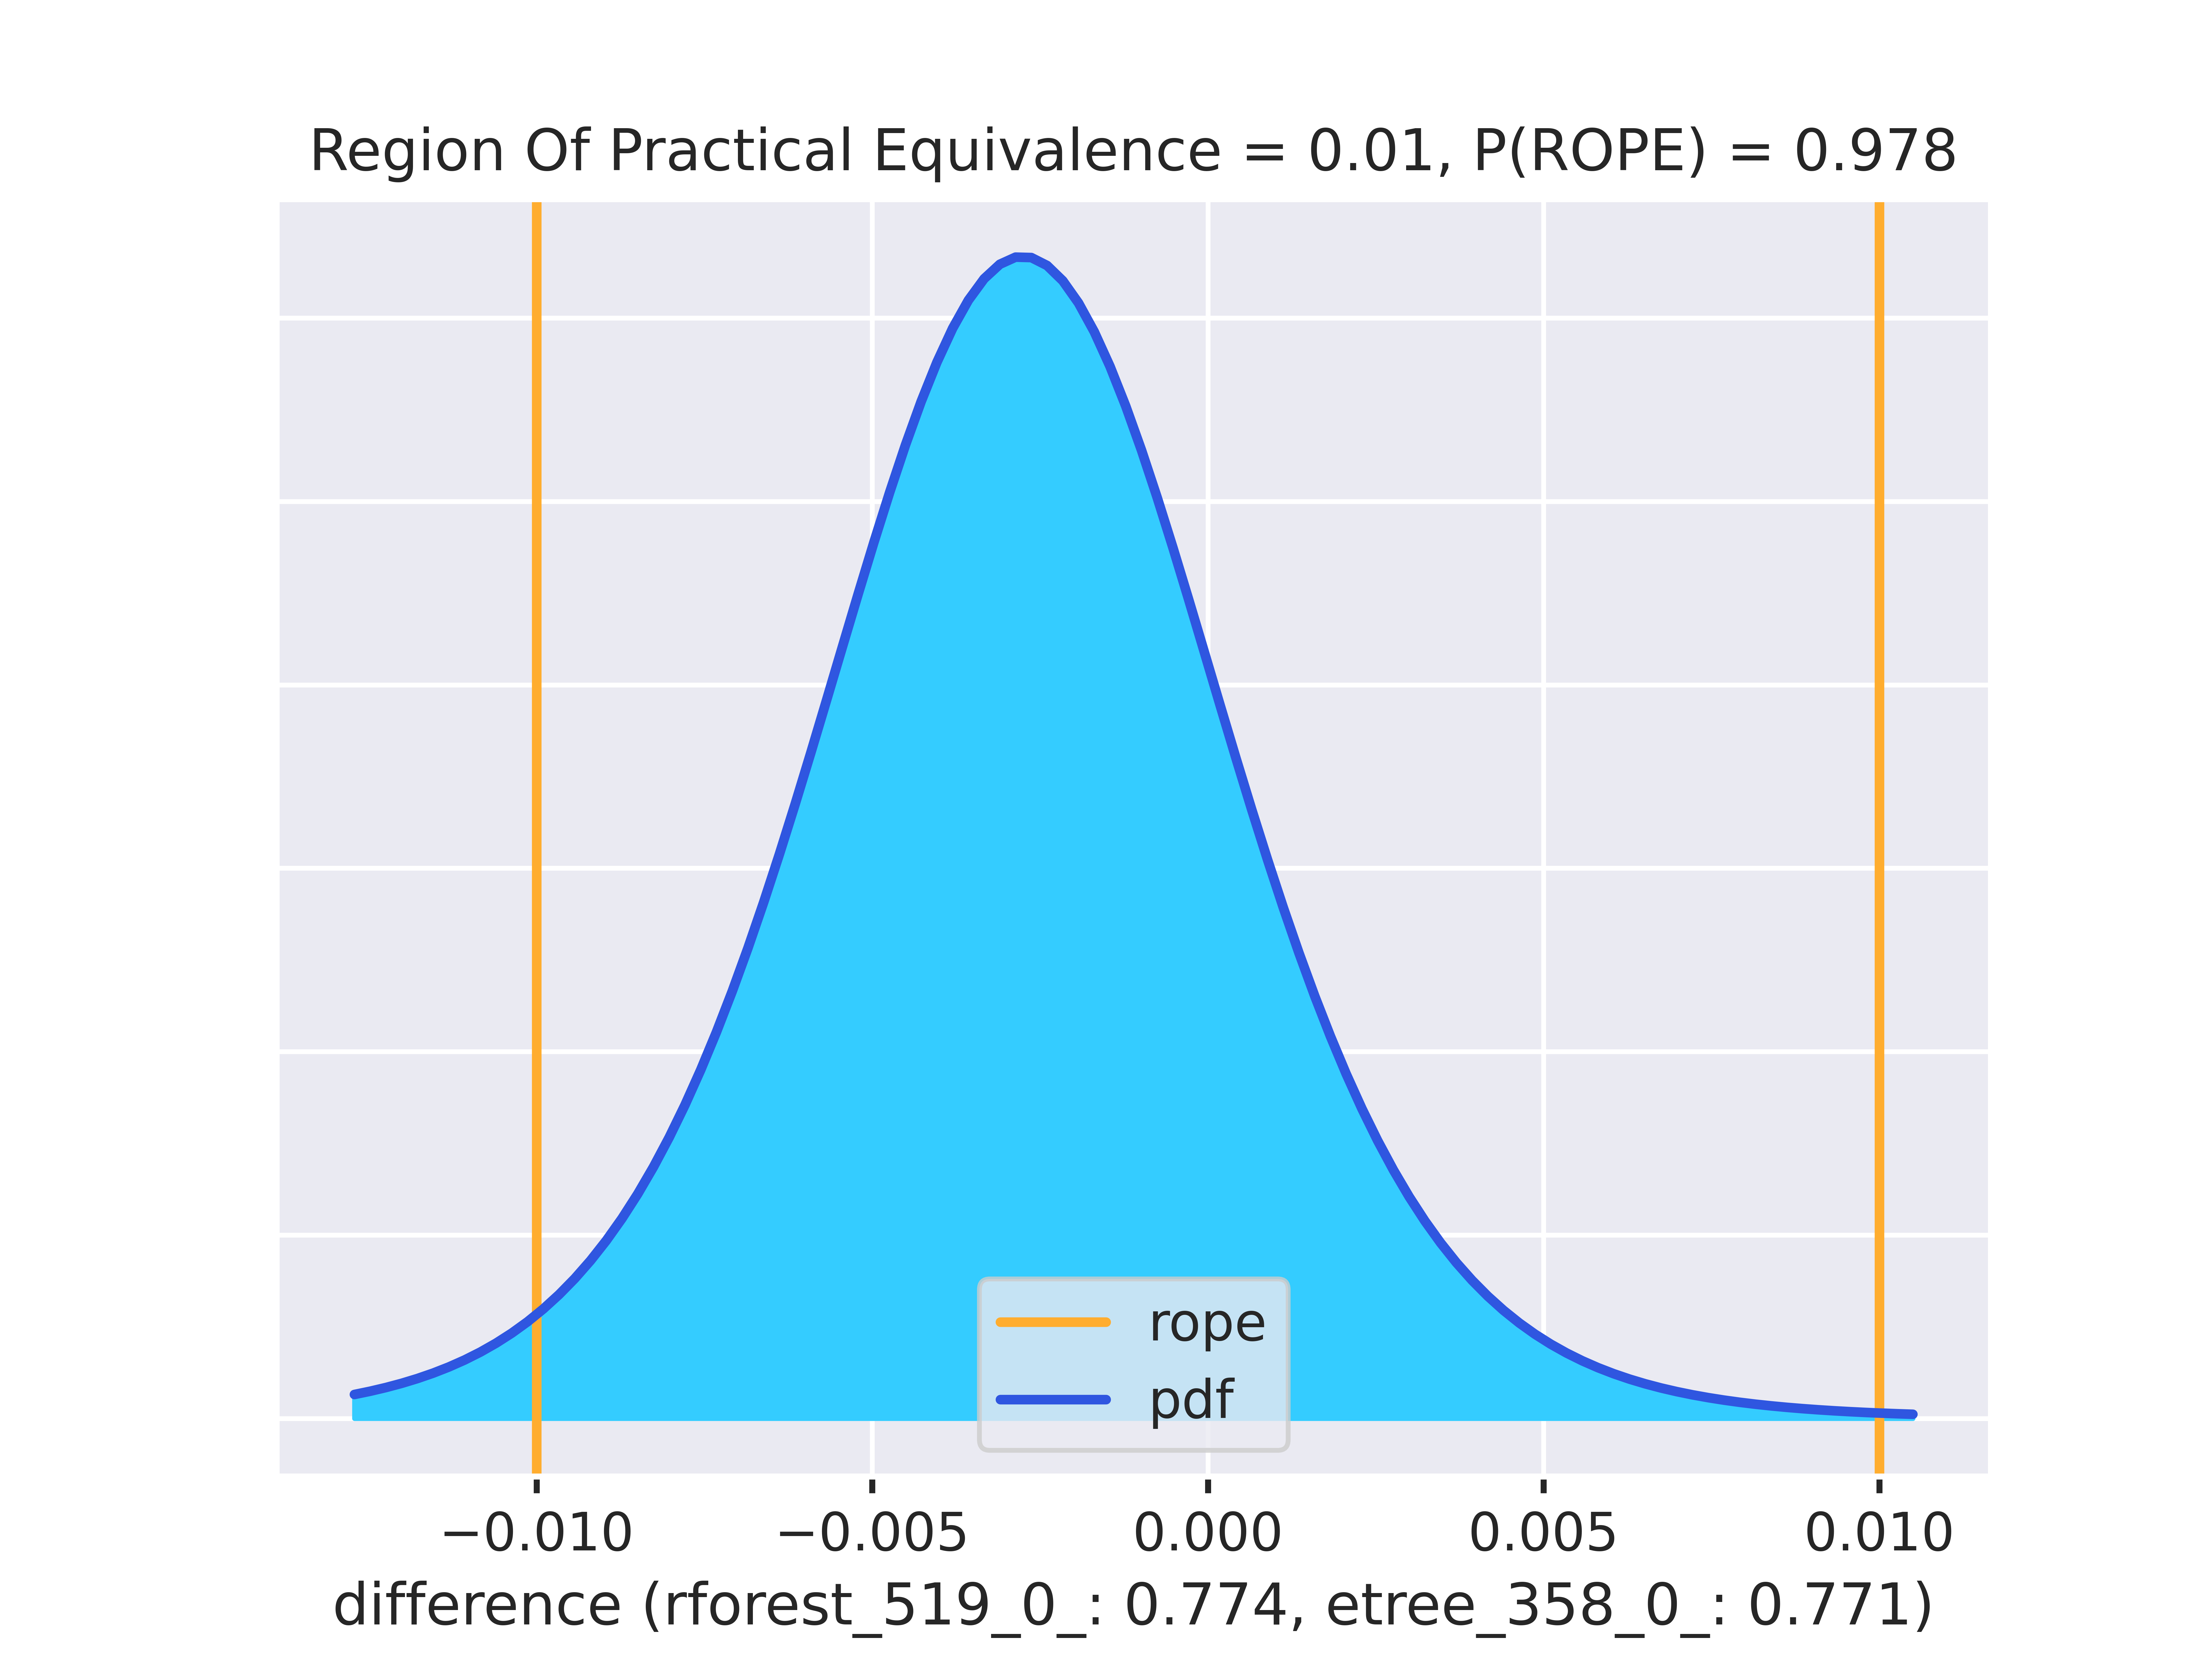
\includegraphics[width=0.5\textwidth]{rope_rforest_519_0__etree_358_0_.png}
                \caption{A probability density function resulting from a Bayesian Signed Rank Test}
                \label{fig:bayes_on_one}
            \end{figure}
            \newline
            \begin{figure}
                \centering
                    \includegraphics[width=0.5\textwidth]{rope_on_two_hxg_boost_531_0__hxg_boost_540_0_.png}
                    \caption{A Bayesian posterior plot resulting from a Bayesian hierarchical correlated t-test}
                    \label{fig:bayes_on_two}
                \end{figure}
                \newline
                The package baycomp \cite{baycomp} is a Python package that implements these Bayesian tests.
                It uses hierarchical for multiple datasets, signed rank for single. 
                The package appears to have been created and refined while this paper was being written \cite{stat2017}

                \subsubsection{ABROCA | Slicing Analysis}

                To understand ABROCA, it is necessary to understand the Receiver Operating Characteristic (ROC).
                The ROC is a function of the false positive rate to true positive rate over the range of threshold values for a predictor.
                originally used to measure performance of radar equipment
                For a more formal exploration of the mathematical properties of the ROC, see \cite{roc2014}.
                
                By integrating over the range of threshold values $[0, 1]$, one finds the area under ROC curve (ROC AUC), a commonly used as a metric to optimize performance of machine learning models.
                By maximizing the ROC AUC, one is maximizing the density of correct predictions while making the threshold value arbitrary.
                It follows that a perfect predictor would reach the theoretical maximum of ROC AUC $= 1.0$, having correct prediction at all threshold values.
                The lowest practical ROC AUC is that of a random predictor, ROC AUC = 0.5. In this case, the model is equally likely to pick correctly or incorrectly at all threshold values.
                
                ABROCA is a metric used to analyze model fairness.
                It was first introduced at 2019 International Learning Analytics and Knowledge Conference \cite{eval2019}.
                To calculate ABROCA, split dataset by feature of interest and obtain the ROC for the model's predictions on each partion of the split dataset.
                Sum absolute values of between-curve area.

                How does this relate to fairness?
                A model that produces equivalent prediction probabilities for the subgroups of the split dataset equally would have ABROCA = 0. 
                Producing the same prediction probabilities would produce the same ROC curves, so there would be no area to sum.
                Hypothesis - Higher ABROCA associated with lower predictive fairness
                \cite{eval2019} found significant differences in fairness when testing different models on a large collection of Massively Open Online Course (MOOC) datasets.
                \begin{enumerate}
                    \item Significant Differences
                    \begin{enumerate}
                        \item Statistical Algorithm
                        \item Featureset Used
                    \end{enumerate}
                    \item Relationship to ABROCA
                    \begin{enumerate}
                        \item Gender Imbalance Ratio
                        \item Curricular Area
                    \end{enumerate}
                    \item Specific Course
                    \begin{enumerate}
                        \item Performance and Fairness
                        \item Not a strict tradeoff with performance and fairness
                    \end{enumerate}
                \end{enumerate}
    
\section{Experimental Architecture}
    \subsection{Dataset}
        \subsubsection{Background}
            The dataset I used in this experiment was made public by the Open University (OU), an online institution based in the United Kingdom.
            The OU provisions one of the largest publicly available LA datasets, known as the Open University Learning Analytics Dataset (OULAD) \cite{oulad}.
            The data comes from 23 presentations (semesters) of 7 different Massive Open Online Courses (MOOCs) (called "modules" by the university) over 2 years and includes demographic, assessment, Virtual Learning Environment (VLE), and course information.
            VLE data is summarized by the number of clicks per course activity per student per day, which amounts to 10,655,280 records associated with 32,593 students.
            In order to be included in the OULAD, a module-presentation had to have over 500 students, at least two different presentations, and utilize the VLE.
            The module also had to have a significant amount of failing students.

            \begin{figure}
                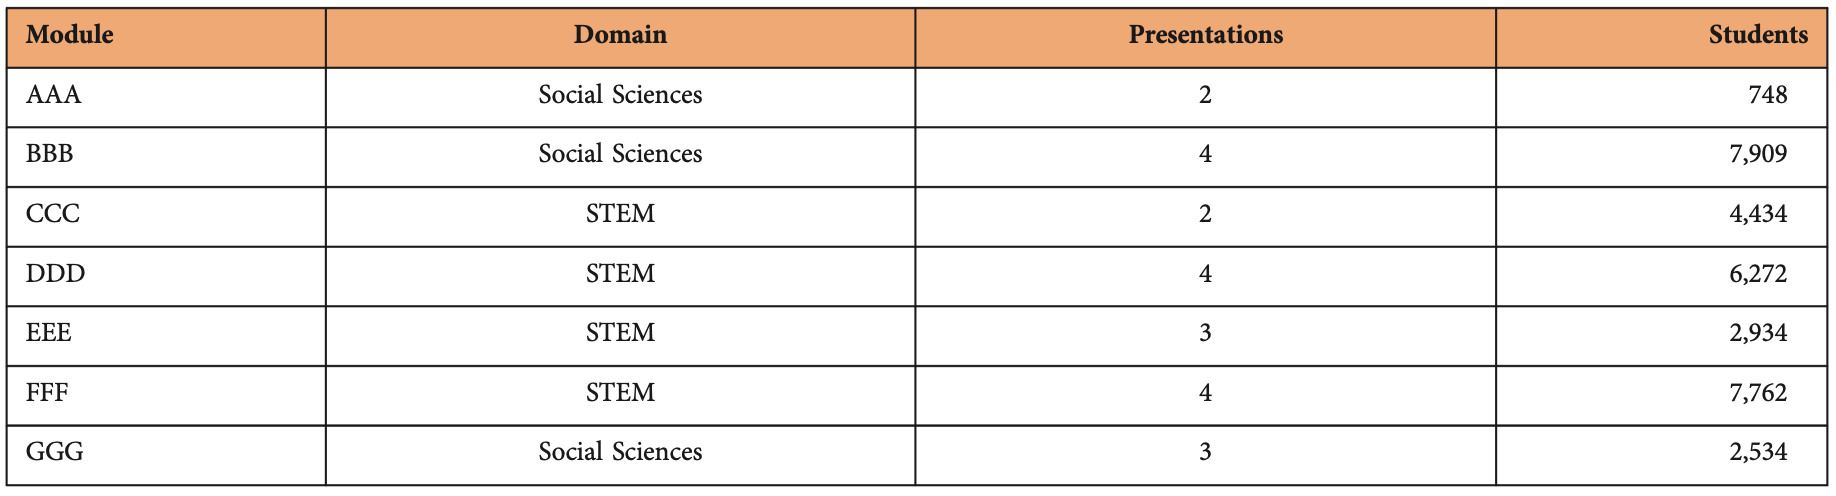
\includegraphics[width=0.5\textwidth]{oulad_students_courses}
                \caption{Module summary and domain information \cite{oulad}}
                \label{fig:oulad_students_courses}
            \end{figure}

        \subsubsection{Description of Tables}
        
            The Open University Learning Analytics Dataset (OULAD) consists of seven tables.
            One table contains student demographic information. 
            A trio of tables describe the courses. 
            There's a table containing the distinct module and presentation codes and a table each for the assessments and Virtual Learning Environment (VLE) activities for each course.
            The three remaining tables bridge the student demographic table with each of the course tables. 
            One table contains the information about course registration.
            One summarizes students' interactions with individual VLE activities on a daily timescale.
            One contains records on students' assessment completion.

            \begin{figure}
                \centering
                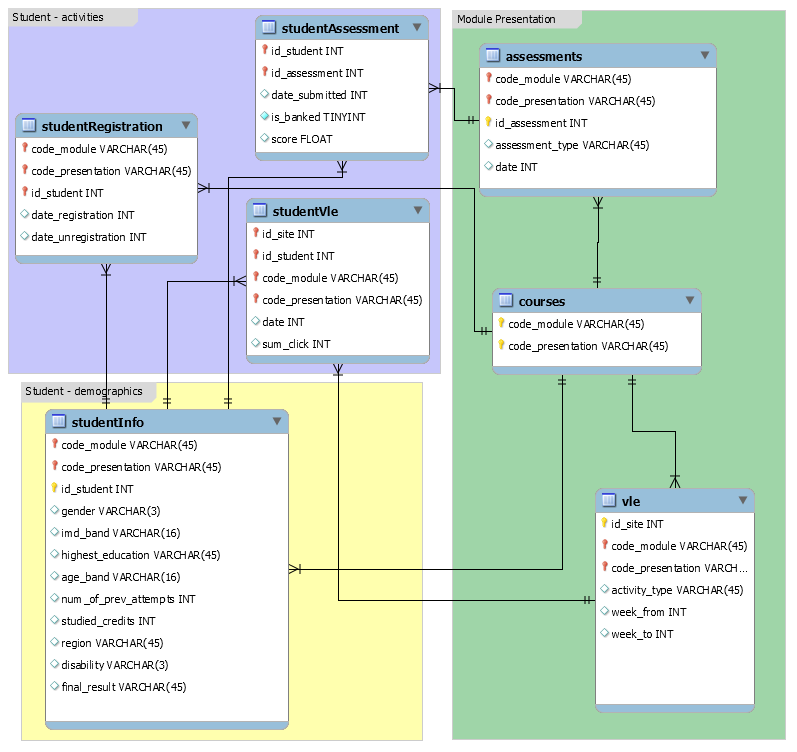
\includegraphics[width=0.75\textwidth]{raw_model}
                \caption{An entity-relationship diagram describing the published dataset \cite{oulad}.}
                \label{fig:oulad_schema}
            \end{figure}
        
        \subsubsection{Comparison to 2015 Data}
            The publishers of the dataset performed an analysis on the distribution of demographic characteristics over time.
            Specifically, they compared a sample of student data from 2015 to the dataset distributions of module CCC, which are from 2013 and 2014.
            The authors performed chi-squared and Wilcox tests to evaluate the null hypothesis that the mean values of these distributions are equivalent.
            At typical significance levels, the null hypothesis cannot be rejected.

            \begin{figure}
                \centering
                \includegraphics[width=0.5\textwidth]{oulad_vs_15}
                \caption{Evaluation of similarity between OULAD and 2015 data for CCC module \cite{oulad}.}
                \label{fig:oulad_vs_15}
            \end{figure}

            A difference between the data from the authors' analysis and the published dataset is the granularity of the information available.
            An anonymization tool was used to obfuscate identifying details in the data while still including specific student demographic information. 
            To illustrate the impact on the data, please see figure xyz.
            \begin{figure}
                \centering
                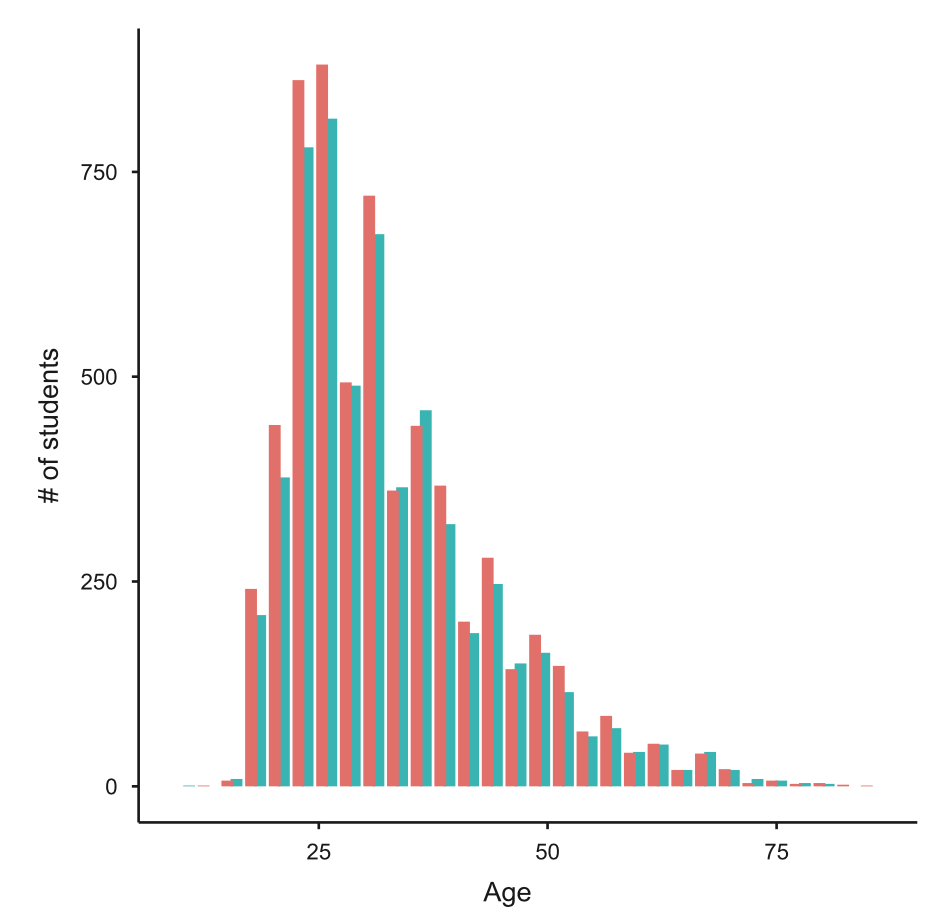
\includegraphics[width=0.5\textwidth]{oulad_15_age}
                \caption{The distribution of student ages for OULAD data (blue) and 2015 data (red) for CCC module \cite{oulad}.}
                \label{fig:oulad_15_age}
            \end{figure}
            \begin{figure}
                \centering
                \includegraphics[width=0.5\textwidth]{age_band_by_student}
                \caption{The distribution of published OULAD age groups \cite{oulad}.}
                \label{fig:age_band_by_student}
            \end{figure}
            
            
            \subsubsection{Other Student Characteristics}
            
            \begin{figure}
                \centering
                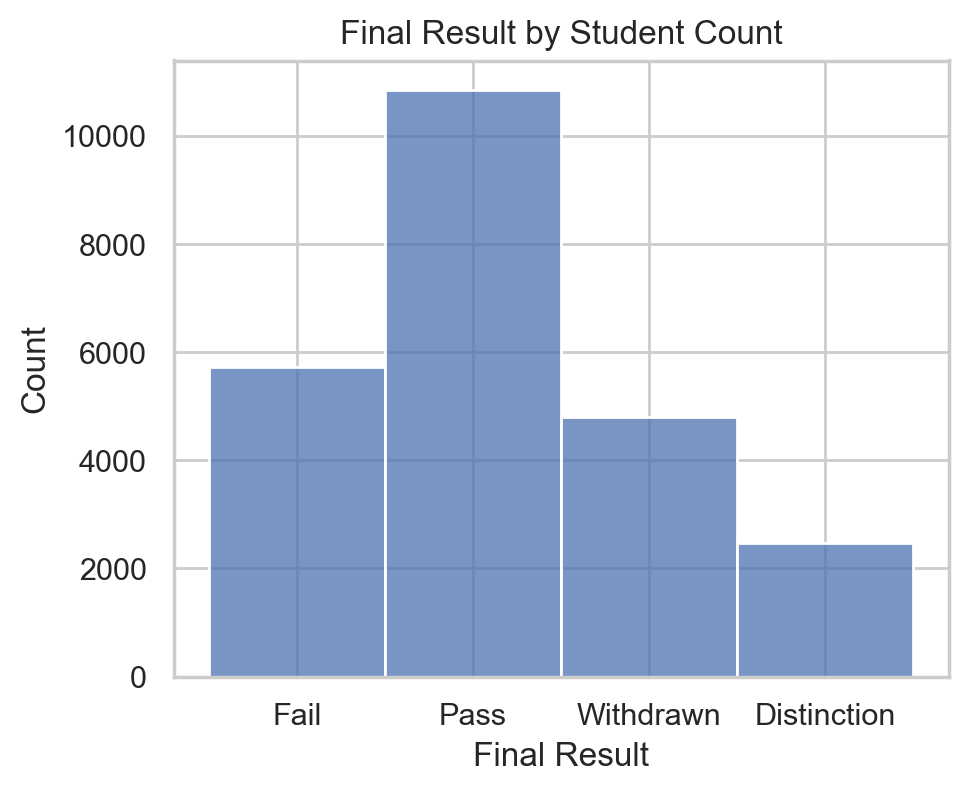
\includegraphics[width=0.5\textwidth]{final_result_by_student}
                \caption{The distribution of published OULAD final module results. \cite{oulad}.}
                \label{fig:final_result_by_student}
            \end{figure}
            \begin{figure}
                \centering
                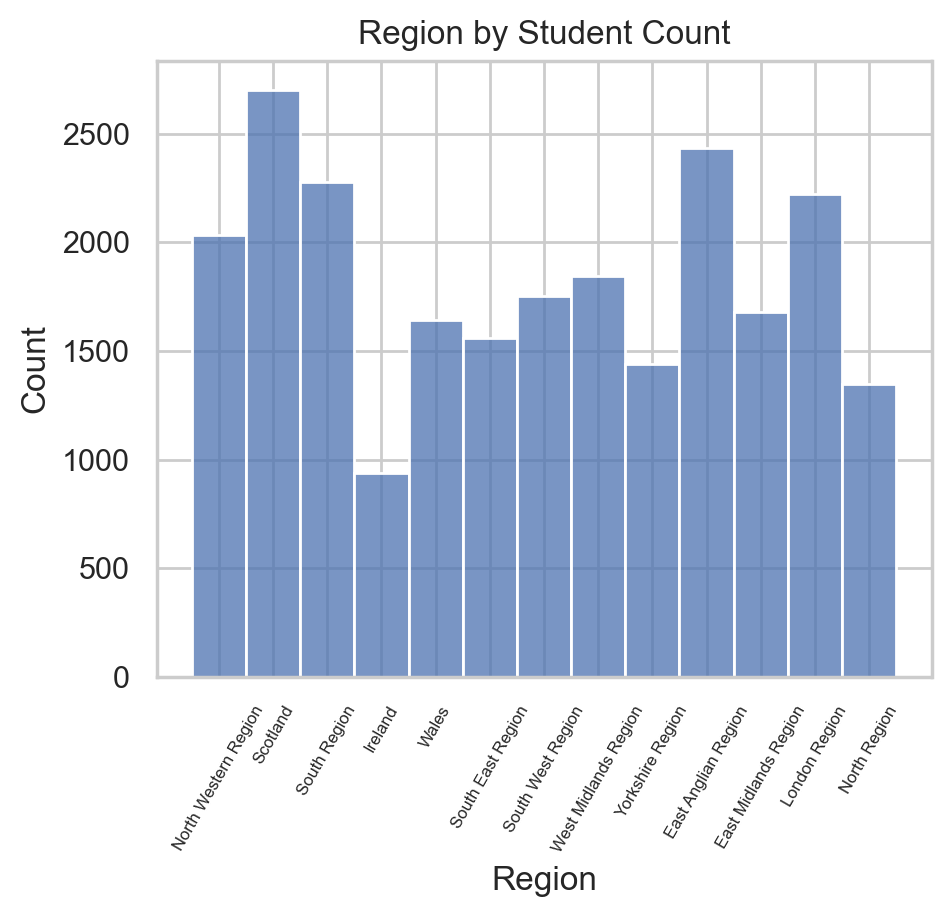
\includegraphics[width=0.5\textwidth]{region_by_student}
                \caption{The distribution of published OULAD final module results. \cite{oulad}.}
                \label{fig:region_by_student}
            \end{figure}
        
        \subsection{Feature Extraction}
        
            \subsubsection{Database System}
                I chose to create a PostgreSQL relational database to organize the cleansing pipeline for this project \cite{postgresql}.
                PostgreSQL is an open source, performant, and reliable relational database system. 
                The clear syntax of Structured Query Language (SQL) for scripting transformations 
                and database operations enabled me to wrangle millions of rows efficiently.
      
            \subsubsection{Flat Files to Main}
                The first step in utilizing the database was ingesting the data.
                I used the Python package pandas to load the Comma-Separated Values (CSV) files into a schema called [landing].
                I then created a schema called [staging] and used SQL to correct and optimize the datatypes of the landing tables.       
                I created a schema called [main] to hold an alternative structure of the data.
                \newline
                The categorical text fields from the staging tables were each given a table to store their distinct values with an integer id as a primary key.
                In the original tables, distinct courses required two text fields for identification.
                In the original student table, the same two fields were necessary, with the addition of an integer student\_id. 
                During the process of transforming the tables into [main], I created a [course\_id] field to identify each module/presentation combination with a single integer.
                I also created a [student\_id] field to identify each individual student record with a distinct integer. 
                Using a single integer field instead of multiple text fields to identify distinct records leads to significant efficiency improvements in storage, memory, and computation.
                While creating new [student\_info] and [course\_info] tables in the [main] schema, I used the new categorical tables to substitute the text values for integer ids.
                This was advantageous not only for the efficiency of utilizing the database, but also because some machine learning models only accept numeric values as input.

            \subsubsection{Main to First30}
                A great deal of research exists which utilizes predictive modeling to enhance the learning experience.
                This information could be used to intervene positively impact students' lives, increasing graduation rates.
                For my project, I decided to predict course outcome.
                This information is most useful when it can be predicted early, which is why I limited the data used for predictions to the first 30 days from the start of the course.
                I also excluded data relating to students who dropped out before the 30 day mark so that their lack of data for certain features wouldn't impact the training process.
                \newline
                I therefore decided to 
                Difference in proportion from Main to First30 for 
                Shown demographics
                Final Outcomes
                Landing to Main Database schema decisions
                Main to First30 Database schema decisions

            \subsubsection{Feature Engineering}
                I built features to use as inputs for the predictive models with inspiration from research and by following intuition \cite{automl2021, early2019}.
                The breadth of feature extraction strategies in research spanned from subject-matter expertise to automation and crowdsources, all of which have their merits.
                
                Some of the features were built in, requiring only the effort to collect to utilize, such as gender and region.
                The major categories of features fall into these four groups: student demographic information, course information, assessment data, and VLE interaction data. 
                The assessment and interaction categories are where most of the "derived" features sit.

                Here's an example of a feature in the VLE activity category that I created when following intuition:
                \begin{figure}
                    \centering
                    \includegraphics[width=1\linewidth]{n_days_active}
                    \caption{The number of distinct days that students interacted with the VLE in the first 30 days}
                    \label{fig:n_days_active}
                \end{figure}

                Here's an example of a feature in the VLE activity category that I built based on on of the expert-created fields in this paper \cite{automl2021}:
                \begin{figure}
                    \centering
                    \includegraphics[width=1\linewidth]{n_total_clicks_by_top_5th_clicks}
                    \caption{The total number of clicks on activities ranked in the top 5th percentile of activities as measured by student clicks}
                    \label{fig:n_total_clicks_by_top_5th_clicks}
                \end{figure}

        
        \subsection{Algorithms and Hyperparameters}
            Hyperparameters are the input parameters for the operation of a machine learning model.
            All of the algorithms and parameter selection components I used are part the Python package scikit-learn \cite{sklearn}
            \subsubsection{Hyperparameter Selection}
                I utilized two different strategies for parameter selection: GridSearch and RandomSearch.
                GridSearch is a brute force strategy where one can specify collections of parameter selections and the cross-validating object will walk through them all. 
                RandomSearch is similar to GridSearch in the way that parameters are mapped out, but selects random combinations from the available ranges.
                Interestingly, one can even set scipy \cite{scipy} random variables as distributions for this cross-validation strategy to pick from during testing. 

                My logic for using both strategies was to first apply wide ranges of parameter combinations for the GridSearch strategy.
                I then used the results from runs to restrict the parameter ranges to those yielding better results.
                Better results in this case refers to higher average ROC AUC while also running in a reasonable timespan. 
                If models were taking longer than 30 minutes to run, I moved the limits of the parameter selection ranges to avoid that when possible.
                The optimization algorithms used to train these models can sometimes not converge to a local (ideally global) minimum, meaning that the predictions will not be the best, which is why restricting the parameter ranges is necessary.

                Once the parameter ranges were sufficiently restricted, I ran my model-generating pipeline using the RandomSearch strategy.
                This can be advantageous because certain combinations of parameter values will never be tried on a reasonable timescale while using a brute force strategy.

            \subsubsection{Algorithms}
                Here is a list of the classification algorithms used in this project along with abbreviations that will appear in later figures. 
                If curious about a particular model or its available parameters, please see \cite{sklearn}.
                The parameterizations of the top two models will be included in the results section of this paper.
                \begin{itemize}
                    \item Decision Tree
                    \item Ada Boosting with decision tree as submodel
                    \item Histogram Gradient Boosting
                    \item Random Forest
                    \item Extra Trees
                    \item K-Nearest Neighbors
                    \item Logistic Regression
                    \item Multi-Layer Perceptron
                    \item Support Vector Machines
                \end{itemize}

        \subsection{Model Pipeline}
            The model generating, training, and testing pipeline was created using scikit-learn components \cite{sklearn} 
            I created separate Python classes that worked together to handle the feature selection, data preprocessing, and parameter selection.
            A class I called ModelEngine orchestrated the process from generation to the logging of results.

            \subsubsection{Data Preprocessing}
                In the data preprocessing pipeline, features were transformed in order to improve their compatibility with making predictions.
                Categorical data was encoded using the "one hot" strategy where each value was pivoted into a Boolean feature.    
                All Boolean features were made numeric.
                Once all features are numeric, the pipeline standardizes each field so that the mean is zero and the variance is one.
                This improves the algorithm's predictive performance by not allowing any of the features to artificially outweigh any other.
                
                If values were missing or null, they were imputed as zeros.
                I decided to impute them instead of exclude them in order to conserve as much data as possible for training.
                
                Any fields with zero-variance are excluded in order to increase computational efficiency.
                With no variance, a field won't be predictive of any result, and will instead just add overhead.
                Another strategy implemented to increase efficiency is Principle Component Analysis (PCA) using a Maximum-Likelihood Estimator (MLE) strategy.
                Similar to the variance threshold, PCA works by reducing model dimensionality in order to reduce model training time, though through a more complex process. 
            
            \subsubsection{Model Training}
                Each model was crossvalidated using a repeated stratified k folds algorithm.
                Each run included five splits and two repeats, totalling ten runs for each model parameterization.
                During training, each model was refit by attempting to maximize ROC AUC.
                The feature that was predicted for the experiment was is\_withdrawn\_or\_fail, simple binary classification.
                The training and testing proportions varied between 0.25 and 0.35.


\section{Results Analysis}
    \subsection{Naive Averaging}
            By simply averaging the results and sorting by performance, we'd miss key details.
            In the below figure, we can see that there is quite a degree of variability on key metrics like predictive performance and fit time.
        \begin{figure}
            \centering
            \includegraphics[width=1\textwidth]{roc_fit_by_mtype}
            \caption{The mean and standard deviation of fit time and ROC AUC by model type}
            \label{fig:roc_fit_by_mtype}
        \end{figure}

    \subsection{Null Hypothesis Significance Testing}
        For the frequentist model comparison, I used non-parametric tests to evaluate model differences.
        I wanted to make as few assumptions as possible about the distribution of the underlying data.
        Additionally, since cross-validation was used, we shouldn't use a t-test \cite{why2009, eval2018}.
        
        A Friedman test \cite{scipy, eval2018} to check for global differences returned a p-value of less than 10e-6, so I turned to the Nemenyi signed rank test \cite{scipy, eval2018} to look at pairwise differences.
        The results can be seen on the below figure, which illustrate one of the major pitfalls of utilizing frequentist methods for model evaluation.
        The wide band of gray shows where we have an inability to reject the null hypothesis at a significance level of 0.05 for the top 69 models.
        That the performance of the models is approximately equivalent is not particularly conclusive. 

        \begin{figure}
            \centering
            \includegraphics[width=0.95\linewidth]{freq_window_20_16_top_100.png}
            \caption{A windowpane plot showing the results of the non-parametric Nemenyi test}
            \label{fig:freq_window_20_16_top_100}
        \end{figure}

    \subsection{Bayesian Region of Practical Equivalence}
        When evaluating model performance using the Bayesian strategy, we find much more conclusive results.
        A Bayesian signed rank test \cite{stat2017, eval2018, time2017} was used to evaluate each pairwise comparison using a ROPE of 0.002.
        I attempted to do all pairwise comparisons with full hierarchical model tests, but the computational overhead for the number of comparisons was too high.
        
        The same top 100 results are shown, but with only two models in the uppermost ROPE, an Extra Tree and a Random Forest model.
        Even looking at the top two approximately-equivalent regions, the top six of seven are tree-based ensemble methods, similar to research.
        Surprisingly there ain't an Ada Boosting model up there.

        \begin{figure}
            \centering
            \includegraphics[width=0.95\linewidth]{bayes_window_20_16_top_100.png}
            \caption{A windowpane plot showing the results of a Bayesian signed rank test using a ROPE of 0.002}
            \label{fig:bayes_window_20_16_top_100}
        \end{figure}

    \subsection{Fairness Though Slicing Analysis}
        I also evaluated the ABROCA statistic and found similar results to \cite{eval2019}.

        First, we have a visualization of two models, each being split two ways.
        In both cases, the extra tree model appears to have better average predictive performance than the logistic regression.
        Both models have a similar ABROCA when it comes to predictions for disabled students, but the extra tree model appears to make predictions less fairly when it comes to gender. 

        \begin{figure}
            \centering
            \includegraphics[width=1\textwidth]{abroca_logreg_271_0_etree_358_0_.png}
            \caption{The ABROCA statistic for two models split by is\_female and has\_disability}
            \label{fig:abroca_logreg_271_0_etree_358_0_}
        \end{figure}

        The top four models happened to be different model types, so I retrained and evaluated the ABROCA for each model on using the data mined from each distinct course.
        The points on each chart represent an individual model's ABROCA score for an individual course, differentiate by color for each course domain. 
        The top two plots show two quadratic regressions that seem to indicate a strong correlation between ABROCA and both the course disabled ratio and course female ratio.
        The bottom two plots appear to show a rather weak correlation between the models' predictive performance and ABROCA.

        \begin{figure}
            \centering
            \includegraphics[width=1\textwidth]{abroca_by_gender_dis}
            \caption{The relationship between ABROCA and demographic balance and mean test ROC AUC for the top four models}
            \label{fig:abroca_by_gender_dis}
        \end{figure}

\section{Conclusion}

    \subsection{Best Models and Features}
        In this experiment, I found that tree-based ensemble methods tended to be the best-performing models on this dataset, with these features.
        The models which performed the best were those that used the entire set of features, not just a subset.
        
    \subsection{Best Evaluation Method}
        Similar to expectations, I found that Bayesian evaluation methods produced the most conclusive answer to the "which model is better question" and suffers from the fewest assumptions or invalidations.

        
    \subsection{Fairness vs Performance}
        I did not see a strong relationship between model predictive performance (as measured by ROC AUC) and ABROCA.
        There did appear to be a strong relationship between demographic ratio and ABROCA.
        This result seems to indicate the ABROCA may be a useful metric in the evaluation of model fairness.
        In addition, this usefulness does not appear to come at the cost of predictive performance.

    \subsection{Future Work}
        To extend this work, additional development of the model generation system could allow for automated hyperparameter distribution optimization.
        More time could be spent refining the feature database and extracting additional predictive features.
        Expend more computing resources on hierarchical comparisons rather than different parameterizations 
        
        A future researcher might evaluate the ABROCA statistic on additional datasets and different categorical splits.
        An attempt could be made to integrate it into the model selection process.
        One might explore if a higher-dimension expression of the calculation holds water.
        More of the mathematical properties of ABROCA could be explored.



        \bibliographystyle{plain}
        \bibliography{paper}
    \end{document}
